To conduct federated learning on smartphones with real-world data,
we rely on the basics of federated learning, communication on smartphones,
and machine learning operations.

\section{General Federated Learning Procedure}

\begin{algorithm}
    \caption{General Federated Learning Procedure}
    \label{algo:general-procedure}
    \ForEach{Training iteration}{
        Distribute the global model to all clients\;
        \ForEach{Client}{
            Train the local model using local training data\;
            Send the trained local model back to the central server\;
        }
        The central server aggregates all local models into a new global model\;
    }
\end{algorithm}

The general procedure of federated learning on mobile devices involves a
distributed system with two parties: the clients and the central server.
The process unfolds through training iterations, with four phases per iteration,
as illustrated in Algorithm~\ref{algo:general-procedure}. In each iteration,
the central server distributes the global model to clients,
who then train the global model locally using their individual data.
Trained local models are sent back to the central server,
and these models are aggregated to generate an updated global model.
This process repeats for successive iterations.
In the context of federated learning on mobile devices,
clients are typically mobile applications on Android or iOS devices,
and the central server is a remote server on the Internet,
as depicted in Fig.~\ref{fig:general-fl}.

\begin{figure}\begin{center}
        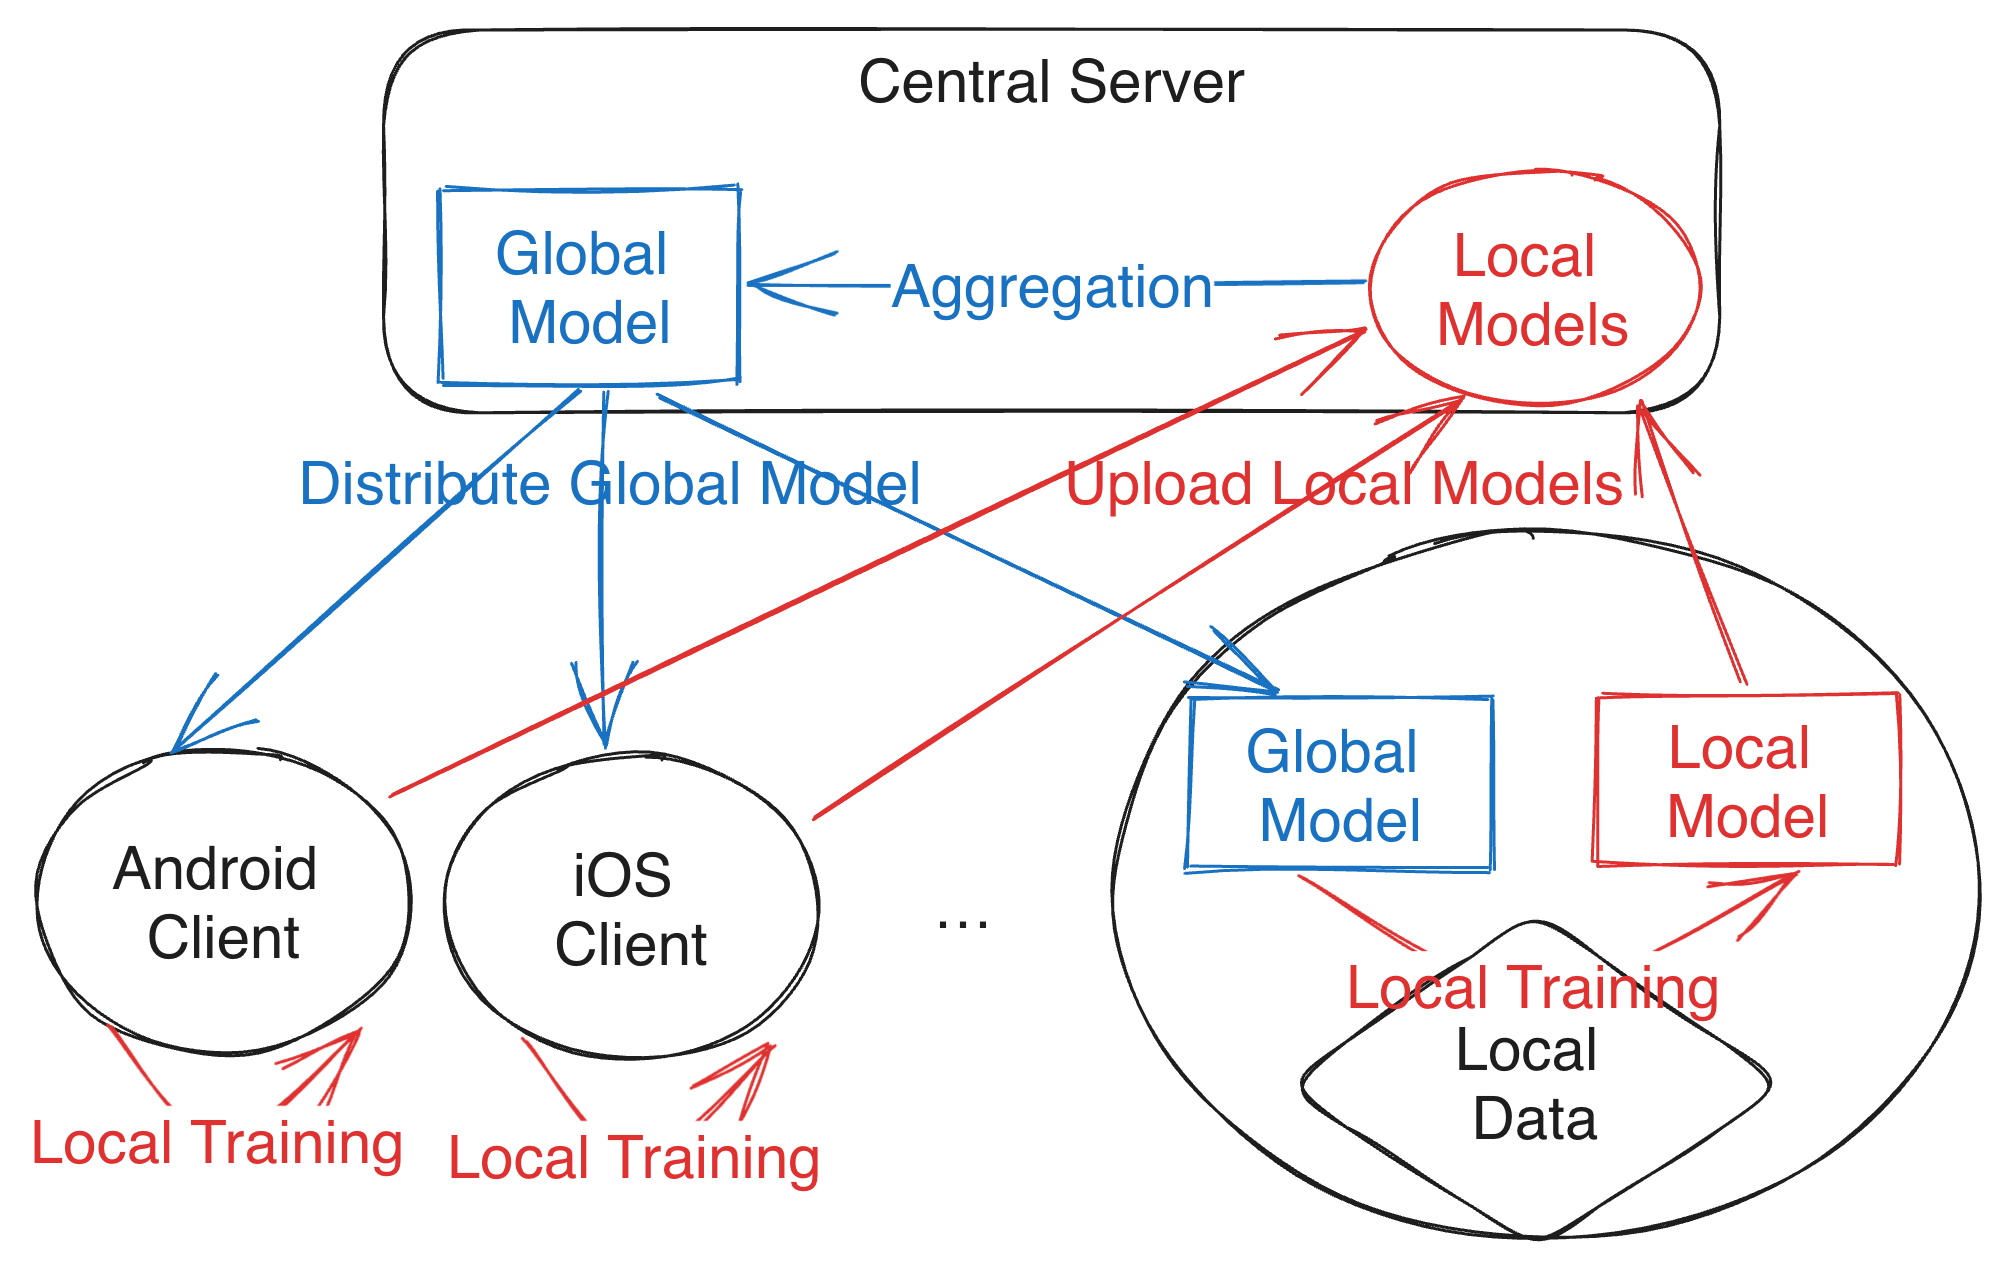
\includegraphics[width=0.7\textwidth]{general_fl.png}
        \caption{General Federated Learning Procedure on Smartphones.}
        \label{fig:general-fl}
    \end{center}\end{figure}

The specific implementations of federated learning on mobile devices may vary,
but they share a common foundation. The FedAvg algorithm,
presented with federated learning itself~\cite{mcmahan2017communication},
stands as the most typical federated learning algorithm. In FedAvg,
a fixed number of $C$ out of $K$ clients are selected for local training in each
iteration.
The local training aims to minimize the loss $L$ of the model for each client's
local data partition $P_k (k \in \{1, 2, \dots, K\})$:
\begin{equation}
    \min_{w_k} L(P_k;w_k),
\end{equation}
starting from the parameters $w^{(t)}$ of the latest global model from the
server, and scheduled for a fixed number of $E$ epochs.
To optimize the global model for the entire training dataset $\bigcup_k P_k$,
FedAvg aims to minimize the weighted average of local losses
\begin{equation}
    \min_{w} \frac{\sum_k |P_k|L(P_k;w)}{\sum_k |P_k|},
    \text{ where }|P_k|\text{ is the size of }P_k,
\end{equation}
by computing the weighted average of local models' parameters
\begin{equation}
    \label{eq:aggregation}
    w^{(t+1)}=\sum_k \frac{|P_k|}{\sum_k |P_k|}w_k^{(t+1)}
\end{equation}
to update the global model, known as model aggregation.
This iteration is repeated until model convergence or experiment termination.
FedAvg has proven effective and practical in various experimental scenarios,
benchmarked against earlier algorithms in data center
settings~\cite{bonawitz2019towards}.

\section{Communication on Smartphones}

A prevalent challenge in implementing federated learning on smartphones is the
fact that clients execute model training on user devices,
which lack direct central control. To overcome this challenge,
federated learning systems commonly integrate remote procedure calls
for communication between clients and the central
server~\cite{tff,he2020fedml,beutel2020flower,patrick2022openfl,madrigal2023project}.
Through remote procedure calls, the server issues instructions to clients,
directing them to execute specific tasks like model training or evaluation,
and clients report back the results.
This mechanism provides developers with substantial flexibility in customizing
scheduling strategies and training algorithms directly on the server.

In practical federated learning implementations,
the gRPC remote procedure call\footnote{\url{
        https://grpc.io/
    }.} emerges as the most popular communication protocol.
It is utilized by \cite{tff,patrick2022openfl} for decentralized simulations,
as well as in \cite{beutel2020flower} for its Flower Protocol.
\cite{madrigal2023project}
offers users the flexibility to choose between representational state transfer
and gRPC. The combination of gRPC and protocol buffers (ProtoBuf)\footnote{\url{
        https://protobuf.dev/
    }.} offers several advantages for communication on mobile devices. ProtoBuf,
with its compact binary data structure representation,
enables efficient transmission,
particularly valuable under the often constrained network conditions of mobile
devices~\cite{popic2016performance}. Additionally,
gRPC and ProtoBuf are language-agnostic,
supporting a variety of programming languages,
easing their adoption on different platforms~\cite{araujo2020performance}.
As gRPC is based on HTTP/2,
it can navigate through restricted firewalls on mobile devices and provides
guaranteed delivery from TCP~\cite{araujo2020performance}.
Its connection-based and bidirectional nature allows the server to actively push
instructions to clients and identify disconnected clients,
valuable for \fedcampus's use case of federated learning on smartphones.

\subsection{On-Device Training Support}

Addressing the imperative of on-device training within federated learning
systems commonly involves the integration of established mobile machine learning
frameworks. Notably,
Google's TensorFlow Lite~\cite{tensorflow2015-whitepaper,abadi2016tensorflow}
for Android emerges as a prominent choice due to its demonstrated flexibility
and maturity in facilitating on-device training.

For Android support in Federated-Learning-as-a-Service (FLaaS) frameworks,
TensorFlow Lite is frequently adopted,
as evidenced by its incorporation in frameworks
like~\cite{kourtellis2020flaas,katevas2022flaas}. Moreover,
TensorFlow Lite serves as a pivotal component in the Android examples provided
by \cite{mathur2021ondevice}, showcasing its versatile applicability.

In contrast, Apple's Core ML~\cite{coreml} experiences less prevalence,
primarily attributed to its perceived lack of user-friendliness.
Although \cite{beutel2020flower} integrates Core ML in its iOS example,
the broader adoption of Core ML in federated learning frameworks remains
limited. Instead, Core ML finds more common usage in specific applications,
such as vision-based quality inspection on iOS~\cite{bharti2022edge}.

However,
challenges emerge when federated learning applications span both Android and iOS
devices, particularly when relying on first-party machine learning frameworks.
TensorFlow Lite and Core ML, being exclusive to their respective platforms,
generate model parameters in distinct representations.
To perform the model aggregation as in Equation~\ref{eq:aggregation},
we require that each client report their model parameters in the same layers and
in the same order.
Rather than changing this requirement or develop separate support tailored for
Android and iOS,
we treat it as a constraint and design our system to satisfy it in
Section~\ref{sec:pipeline}.

\section{Machine Learning Operations}

% TODO: Improve this and cite.
Machine learning operations (MLOps) is a set of practices similar to
development operations (DevOps).
In development operations,
the software development process and the deployment process are integrated,
so that new software changes made by the development team can be
automatically deployed into production.
Similarly, in machine learning operations,
changes in the machine learning algorithms can be automatically deployed into
production.
Machine learning operations is desirable when the development velocity on
the machine learning algorithms is high,
and feedbacks from the production environment are important to improve
the machine learning algorithms.
